\documentclass[a4paper,11pt,openany]{report}
\usepackage[utf8]{inputenc}
\usepackage[english]{babel}
\usepackage[font=small,labelfont=bf, textfont=it]{caption}
%\usepackage[bottom=2cm, left=2.5cm, right=2.5cm]{geometry} % to change padding
\usepackage{verbatim}
\usepackage{subcaption} % for multi figure
\usepackage{enumitem} % -- label item
\usepackage{tabularx}
\usepackage{color}
\usepackage[usenames, dvipsnames]{xcolor} % color
\usepackage[framemethod=TikZ]{mdframed} % box
\usepackage{listings} % code
\usepackage{minted} % code
%\usepackage{amsmath} % align* maths
\usepackage{wrapfig}
\usepackage[section]{placeins} % float inside subsection
\usepackage[bookmarks, hidelinks]{hyperref} % clickable links
\usepackage{graphicx} % includegraphics
\usepackage{indentfirst}

\setlength\parindent{0pt}
\setlength{\parskip}{1em}

\renewcommand\thesection{\arabic{section}} % start section from 1
\setcounter{tocdepth}{2} % display subsection
\setcounter{secnumdepth}{3} % number subsubsection

% \title{Internet Security \& Privacy\\Seminar -- Report\\\vspace{10pt}\textbf{CSRF attack: even Google was vulnerable.}}
% \author{Quentin Lemaire \& David Kufa\\Group 26}

\newcommand{\csrf}{\textit{Cross-Site Request Forgery}}


\begin{document}

  % first page
 \begin{titlepage}
  \centering
  \vspace*{\stretch{1}}
  \vfill
    {\bfseries\Large{
	Internet Security \& Privacy\\
	Seminar -- Report}
    }    
  \vfill
  \vfill
    \Huge{\textsc{CSRF attack: even Google was vulnerable.}}
  \vfill
      \Large{\textsc{David Kufa} \& \textsc{Quentin Lemaire}}
    \\
  \vspace{0.4cm}
    Group 26
  \vfill
  \vfill
    % \includegraphics[width=0.22\textwidth]{kth.jpg}
    KTH Royal Institute of Technology
  \vfill
    \today
  \vspace*{\stretch{1}}
\end{titlepage}

% abstract
\begin{abstract}
  \csrf{} (CSRF) -- often spelled ``sea surf'' -- is a well-known web attack which has 
  been discovered in 2001. The \textit{Open Web Application Security Project} (OWASP \cite{owasp}) 
  ranked CSRF as the 8th\footnote{In 2007 \& 2010 OWASP's tops ten, CSRF was at the 5th position 
  (\url{https://www.owasp.org/index.php/Top_10_2007} \& \url{https://www.owasp.org/index.php/Top_10_2010}).} 
  vulnerability in the top 10 of the most critical web application security risks in 2013~\cite{owasp_top_ten}.
  
  CSRF attack consists in creating (forging) fake HTTP or HTTPS\footnote{TLS encrypts 
  information between the client (browser) and the server in order to prevent sniffing 
  in untrusted networks and man in the middle attacks but it doesn't protect from 
  legitimate requests.} requests on the user's behalf. It utilizes the lack of knowledge 
  of the victim to build the request and get information with their credentials (as if 
  the user really wanted to execute this request). In order to succeed, the victim must 
  be connected (authenticated) to the service (website) where there is the vulnerability. 
  Then, an attacker will have to fool the victim in order to build the fake request (with 
  social engineering for instance).
  
  During this seminar, we wanted to get a better understanding of the security breaches 
  involved in CSRF attack. The most interesting part consisted in the comprehension of 
  the surface of attack, how this attack can be done and where does it come from. It 
  was also important to understand what kind of information an attacker could steal or 
  affect on the user's behalf thanks to this attack. Furthermore, it was relevant to study 
  different ways of detecting the vulnerability and how to protect web servers from this 
  attack.
  
  In a second part, we focused our attention on concrete applications of CSRF vulnerabilities. 
  Lots of companies were affected in the past and we decided to deal with Google well-known 
  stories about CSRF. Indeed, 2 different vulnerabilities were discovered in 2007 concerning 
  Gmail \footnote{\url{https://mail.google.com/}} email service.
  
  Finally, we implemented a small webapp with different services, either vulnerable or protected 
  from CSRF attack. This webapp associated with an attacker website, both developped from scratch, 
  outline different practical examples of the attack and different ways to prevent it.
  \end{abstract}
  
%   \begin{enumerate}
%    \item CSRF: how it works ? Implementation of a vulnerable web service.
%    \item CSRF: how to prevent it ? Implementation of a protected web service with different methods of protection.
%    \item Some stories about CSRF: 2 Google vulnerabilities in 2007.
%    \begin{itemize}
%     \item Contact list spoofing: it was possible to retrieve all the contact list of an user~\cite{gmail_contact_list_csrf, gmail_contact_list_csrf2}.
%     \item Email filter hijacking: it was possible to forward all email of an user to another selected email address~\cite{gmail_hijack_csrf, gmail_hijack_csrf2}. This attack had a great impact on Gmail users trust.
%    \end{itemize}
%   \end{enumerate}

\tableofcontents{} % toc
\clearpage % leave a page
\setcounter{page}{1} % init counter page

  % TODO part1: overview of CSRF
  % TODO     * Description & Identification
  % TODO     * Exploitation
  % TODO     * Recommandations: how to prevent CSRF ?
  
  % TODO part2: Google stories: how ? impact ?
  % TODO     * Contact list spoofing
  % TODO     * Email filter hijacking

  \section{Introduction}
  
  This report is split in two different parts. First, it deals with \csrf{} (CSRF) attack in 
  a theoretical and practical way. Academic examples and explanations describe and explore 
  different aspects and subtilities of CSRF attack. The second part of this report is about concrete 
  uses (in ``real life'') of CSRF breaches with 2 use cases about Google Gmail service.

  \section{Overview of CSRF}
  
  For each kind of WEB vulnerabilities, it is important to know how to detect them and 
  how to prevent them. We will explain in more details what is CSRF attack, how to 
  identify and exploit CSRF vulnerable services and finally how to protect these services. 
  Every explanations will be followed with example from a web application we developed. 
  This web application provides different services in order to manage and store a list of 
  interests (hobbies). More explanations from the technical documentation can be found 
  in appendix~\ref{app:practical_documentation}.
  
  \subsection{Description \& Identification}
  
  % TODO explain how CSRF work (reuse abstract)
  
  \subsection{Exploitation}
  
  % TODO example with webapp
  
  \subsection{How to prevent it ?}
  
  % TODO example with webapp
  
  \subsubsection{Tokens}
  
  \paragraph{Session token}
  It is possible to use a session token which is a ``random'' number generated at the beginning 
  of the user's session (authentication). The token is sent by the server in every forms (for POST 
  requests) as a hidden HTML input (as shown in figure~\ref{figure:session_token_client}) or URL 
  (for GET requests) as a parameter. This number must be sent by the browser in every requests in 
  order to achieve a service. In order to avoid replay attack, it is important to change this token 
  after each use of service. Token must be stored in the user's session on the server to check its 
  validity (as shown in figure~\ref{figure:session_token_server}).
  
  \begin{figure}[h!t]
  \begin{minted}[linenos]{html}
<form method="POST" action="?p=account&action=delete">
    <input type="hidden" name="csrf_token" value="5XWla[...]hHNPpXs=" />
    <input type="submit" value="I'm sure I want to delete my account" />
</form>
  \end{minted}
  \caption{Example of a session token (client side)}
  \label{figure:session_token_client}
  \end{figure}
  
  \begin{figure}[h!t]
  \begin{minted}[linenos]{php}
<?php
$token = $_POST['csrf_token'];
$valid_request = $token === $_SESSION['token'];
?>
  \end{minted}
  \caption{Code to check session token (server side)}
  \label{figure:session_token_server}
  \end{figure}
  
  \paragraph{Signed token} % show code as example (using HMAC)
  It is possible to use a Hash based Message Authentication Code (HMAC) in order to ``sign'' 
  generated token. With a private secret only known by the server, tokens are signed using 
  HMAC and this hash is concatenated to the token before sending it to user (in a hidden 
  HTML input as shown in figure~\ref{figure:signed_token_client}). This signed token avoid 
  storage of tokens in session but this method has several drawbacks like ``golden'' token. 
  Indeed, if the token is stolen (somehow), it can be reused on the user's behalf. In order 
  to prevent this kind of event to happen, it is possible to append a timestamp (time to 
  leave) after the token value. HMAC will protect the timestamp from modification (integrity 
  check) so there is no need to encrypt it. Example to build and check tokens is displayed 
  in figure~\ref{figure:signed_token_server}.
  
  \begin{figure}[h!t]
  \begin{minted}[linenos]{html}
<form method="POST" action="?p=interests&action=add">
    <input type="hidden" name="csrf_token" 
        value="WQJCXDUivLPd1r5OLW[...]OYdw==$f75bfabe1[...]04394e6b" />
    [...]
    <input type="submit" value="Create interest" />
</form>
  \end{minted}
  \caption{Example of a signed token (client side). The value is split in 2 parts: the first part 
  (before \$ symbol) contains the token. The second part (after \$ symbol), there is the HMAC which 
  will let the server check integrity of the token.}
  \label{figure:signed_token_client}
  \end{figure}
  
  \begin{figure}[h!t]
  \begin{minted}[linenos]{PHP}
<?php
const SECRET_KEY = 'a0e605ee21f0b7bdd85ff2edb8177dcf'; // 16 bytes key
const SEPARATOR = '$'; // not base64 chars i.e. not from [0-9a-zA-Z/=+]

public static function generate_signed_token($size = 64) {
    $token = self::generate_token($size); // base64 token
    $signed_token = self::sign_token($token);
    return $token . self::SEPARATOR . $signed_token;
}

private static function sign_token($token) {
    return hash_hmac('sha512', $token, self::SECRET_KEY);
}
  
public static function check_signed_token($received_token) {
    list($token, $signature) = explode(self::SEPARATOR, $received_token); // split
    $signed_received_token = self::sign_token($token); // sign received token
    return $signature === $signed_received_token; // compare with signature
}
?>
  \end{minted}
  \caption{Code to check a signed token (server side).}
  \label{figure:signed_token_server}
  \end{figure}
  
  \subsubsection{Challenges}
  
  \paragraph{Double authentication} % retype password
  \paragraph{CAPTCHA} % find a text inside a picture (similar to token)
  
  \subsubsection{Other protections}
  
  Recommendations described above are not exhaustive. It is possible to combine them in order to increase 
  the security of the application against CSRF attack.
  
  
%   We are aware that it will be difficult to make a demonstration during the oral presentation 
%   because we don't have too much time for this. That's why we won't show our practical part 
%   during the oral presentation but we may use this part as a common thread for our explanations. 
%   
%   Technically speaking, we will implement a small platform using either \textit{Apache 2.4}\footnote{\url{https://httpd.apache.org/}} or \textit{nginx}\footnote{\url{http://nginx.org/}} as a web 
%   server. As a database, we can either use \textit{MySQL}\footnote{\url{http://www.mysql.com/}} or \textit{PostgreSQL}\footnote{\url{http://www.postgresql.org/}} which are relational databases. We own a small \textit{Raspberry Pi}\footnote{\url{https://www.raspberrypi.org/}} 
%   in which we can develop this platform. It will contain several things:
%   \begin{itemize}
%    \item An authentication system, which is part of the attack, an attacker wants to forge request on the behalf of an user, and he or she has to be connected.
%    \item A vulnerable service: a GET or POST service which updates data about the user (password for instance).
%    \item Some protected services with different protection methods:
%    \begin{itemize}
%     \item CSRF tokens known from the server and the client ;
%     \item Signed tokens with a private secret (only known by the server), this is a simple way to avoid saving and storing tokens but this method has several drawbacks like ``golden'' token (if the token is stolen, it can be reused on the user's behalf). This protection method will use what we've learnt from the symmetric encryption and hashing lectures of this course ;
%     \item Confirmation pop-up ;
%     \item Session information in URL in order to ``randomize'' the URL request as much as possible ;
%     \item \textit{HTTP-REFERER} check but since this value comes from the client (which has been tricked), it can't be trusted.
%    \end{itemize}
%   \end{itemize}
%   
%   According to the programming language, we don't have any preferences. Python seems to be very easy to 
%   compute with libraries like \textit{Flask}\footnote{\url{http://flask.pocoo.org/}} or 
%   \textit{Django}\footnote{\url{https://www.djangoproject.com/}} (but we won't use Django because it 
%   already provides tools against CSRF attack). We can also build a small website with PHP from 
%   scratch. This language provides lots of database integration tools\footnote{PHP provides classes as \textit{PDO} (\url{http://php.net/manual/en/book.pdo.php}) 
%   which protects from SQL injections thanks to prepared statements but this is not the point of this seminar.} 
%   and session management.
%   
%   Finally, in order to build reports and presentations (beamer), we will use \LaTeX{} and we will utilize a version control system to 
%   version and backup our code (\textit{Git}).
  

  \section{Google, vulnerable to CSRF in 2007}
  
  % TODO put in context
  
  \subsection{Contact list spoofing}
  % TODO
  \subsubsection{Description}
  % TODO
  \subsubsection{Exploitation}
  % TODO
  \subsubsection{Impact}
  % TODO
  
  
  \subsection{Email filter hijacking}
  % TODO
  \subsubsection{Description}
  % TODO
  \subsubsection{Exploitation}
  % TODO
  \subsubsection{Impact}
  % TODO
  
  \subsection{Comparison}
  % TODO
  
  
  
  \section{Conclusion}
  % TODO conclusion

  
  % TODO all \nocite{}
  
% appendix
\appendix
\addtocontents{toc}{\protect\setcounter{tocdepth}{-1}}

\chapter{Practical documentation} \label{app:practical_documentation}
% TODO

\section{Introduction}
The webapp developed is a small web application delivering different features 
in order to store and manage a list of interests. It provides authentication and 
interests'management. It has been developed from scratch with \textit{Apache 
WEB server 2.4}\footnote{\url{https://httpd.apache.org/}} and \textit{PHP 5.6}. 
The database used is \textit{MySQL 5.5}\footnote{\url{http://www.mysql.com/}} with 
\textit{InnoDB} engine.

\section{Specifications}

\subsection{Description}

In this web application, users can register and log in from their browser. As soon as 
they registered with a login, a password and an email, they are able to connect to 
the application. Once connected, the user has different possibilities. He or she can 
change their account settings like the email attached to the account. A service lets the 
user delete his or her account. He or she can also add new interest to their list of 
interests. An interest is composed of a name and a description which is optional. It is 
possible to remove interests from the list (unbind) and add (bind) as many interests as 
possible.

Some services are protected from CSRF attack, some aren't. An exhaustive list of implemented 
services is described below.

\subsection{Services}

Different entities are parts of the web application's model. Here is an exhaustive list of implemented 
services, each one of them are prefixed with either ``[public]'' or ``[private]''. ``[public]'' means that 
service is accessible from the web (with a URI) and ``[private]'' means that service is not accessible from 
the web.
\begin{description}
 \item[User] this entity provides functions and methods related to user management
 \begin{itemize}[label=--]
  \item {[}public{]} Register a user with a login, a password and an email
  \item {[}public{]} Login a user with a couple (login, password)
  \item {[}private{]} Check \& hash password
  \item {[}public{]} Change user's email: \color{red}{vulnerable to CSRF attack}\color{black}{}
  \item {[}public{]} Disconnect the user
  \item {[}public{]} Delete user account: \color{green}{protected against CSRF attack}\color{black}{}
 \end{itemize}
 
 \item[Interest] this entity provides functions and methods related to interest management:
 \begin{itemize}[label=--]
  \item {[}public{]} Add an interest: \color{green}{protected against CSRF attack}\color{black}{}
  \item {[}public{]} Remove an interest: \color{red}{vulnerable to CSRF attack}\color{black}{}
  \item {[}private{]} Bind an interest with a user
  \item {[}private{]} Unbind an interest with a user
  \item {[}public{]} Get user's interests
  \item {[}private{]} Get all interests
 \end{itemize}

 \item[CSRF] this entity is not directly related to the web application but it contains the 
 implementation of CSRF protection functions and attributes:
 \begin{itemize}[label=--]
  \item {[}private{]} Secret key
  \item {[}private{]} Generate token
  \item {[}private{]} Check token
  \item {[}private{]} Sign token
  \item {[}private{]} Generate a signed token
  \item {[}private{]} Check a signed token
 \end{itemize}

\end{description}

\subsection{Database}
The database schema is composed of the two main entities of the web application:
\begin{itemize}
 \item Users
 \item Interests
\end{itemize}
Each attributes, table names and relations are defined in figure~\ref{figure:database}.

\begin{figure}[h!t]
  % trim=left bottom right top
  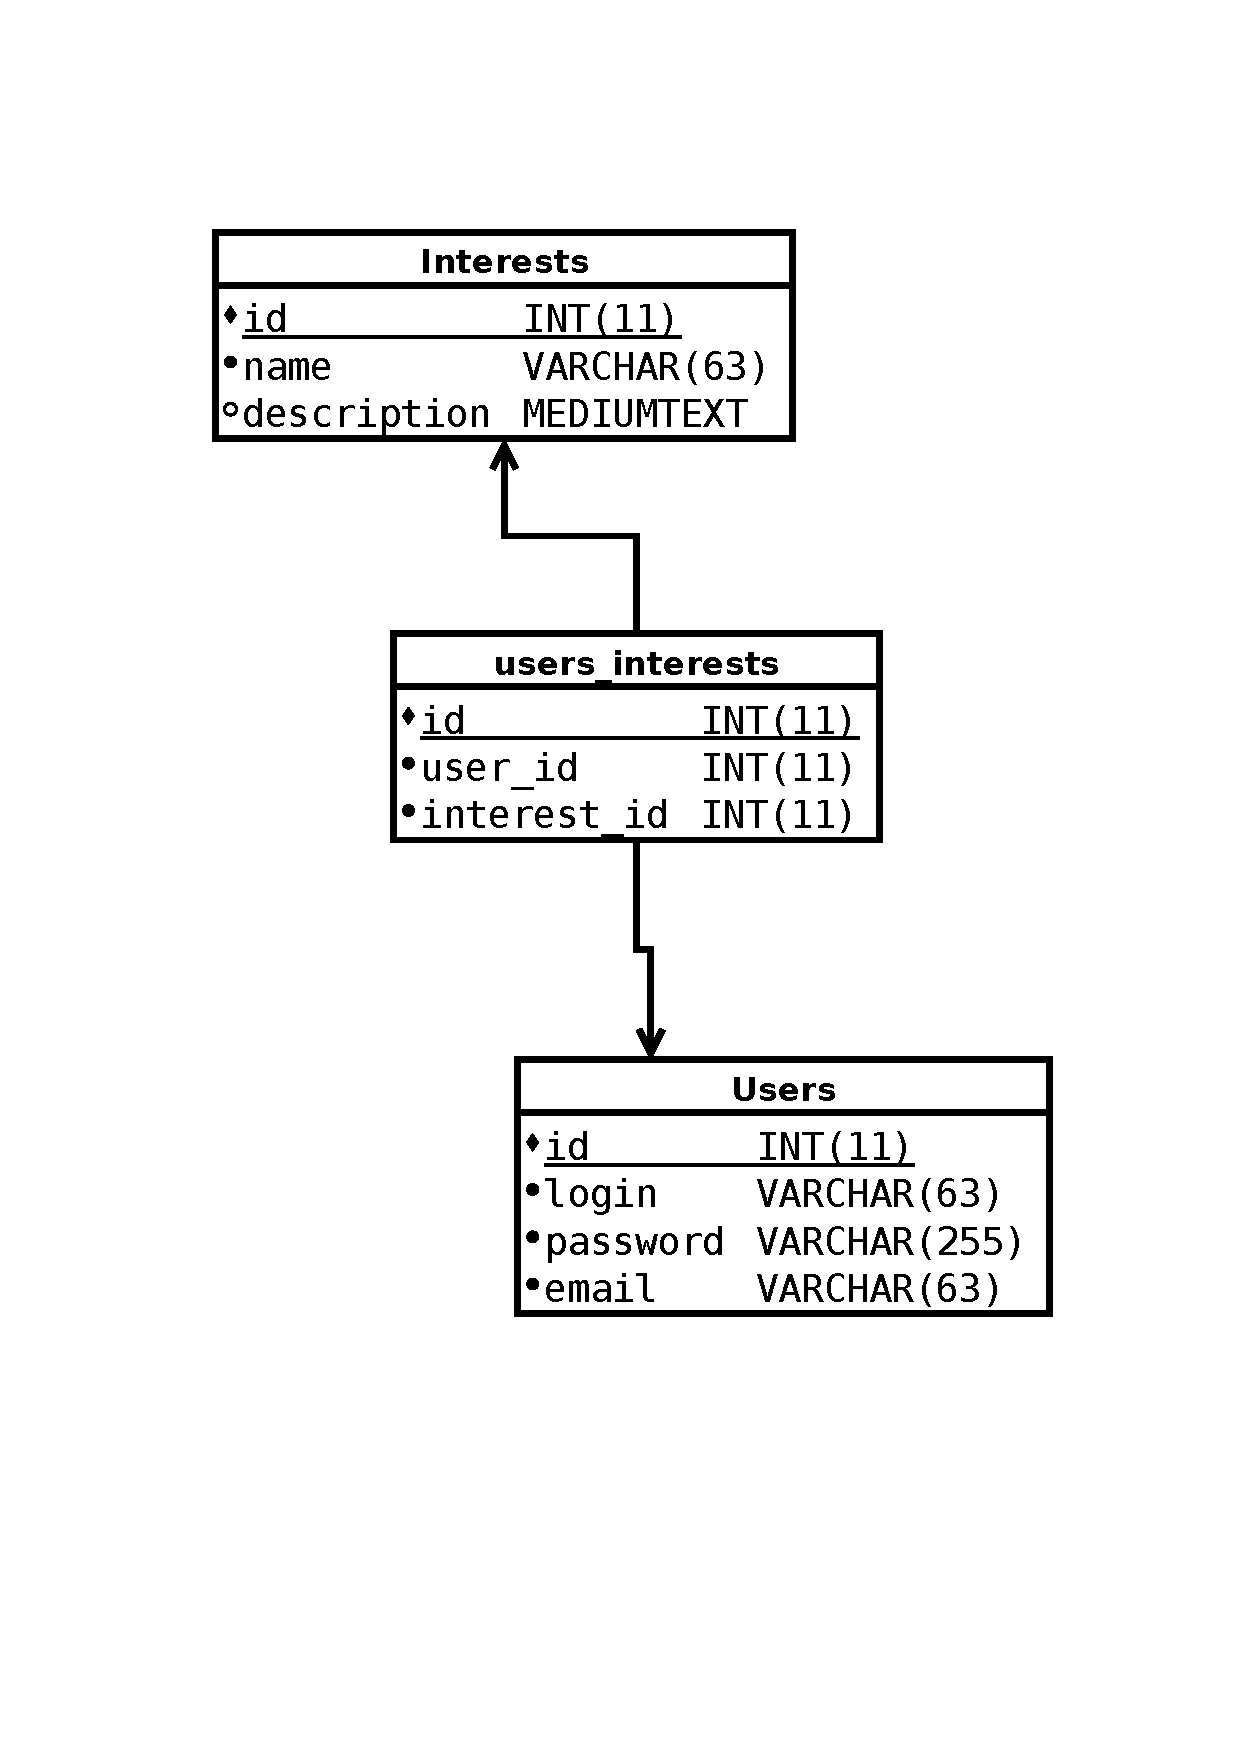
\includegraphics[trim=0 200 0 110,clip,width=\textwidth]{database.pdf}
  \caption{Database diagram. Arrows represent foreign keys. Extra information: ``login'' in ``Users'' table is UNIQUE.}
  \label{figure:database}
\end{figure}
  
  
\chapter{Web application's screenshots} \label{app:screenshots}
% TODO

\begin{figure}[ht!]
  \begin{center}
    \fbox{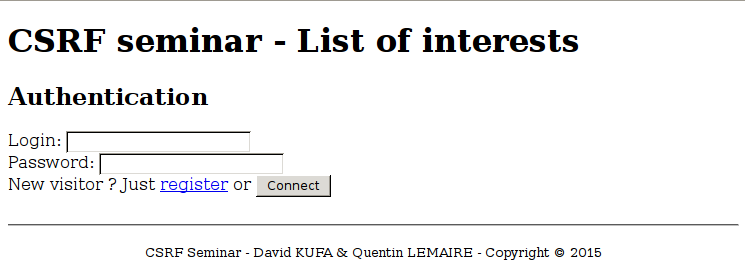
\includegraphics[width=.9\linewidth]{screens/login.png}}
    \caption{Login page}
    \label{figure:login}
  \end{center}
\end{figure}

\begin{figure}[ht!]
  \begin{center}
    \fbox{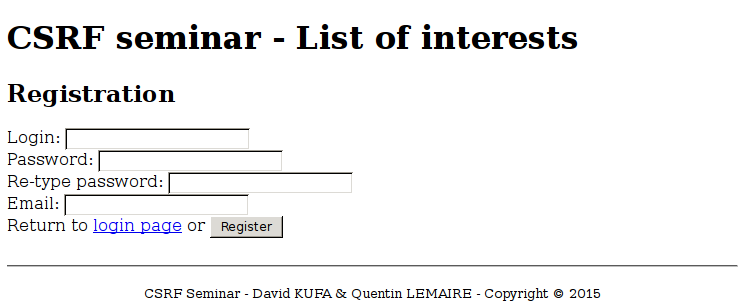
\includegraphics[width=.9\linewidth]{screens/register.png}}
    \caption{Register page}
    \label{figure:register}
  \end{center}
\end{figure}
  
\begin{figure}[ht!]
  \begin{center}
    \fbox{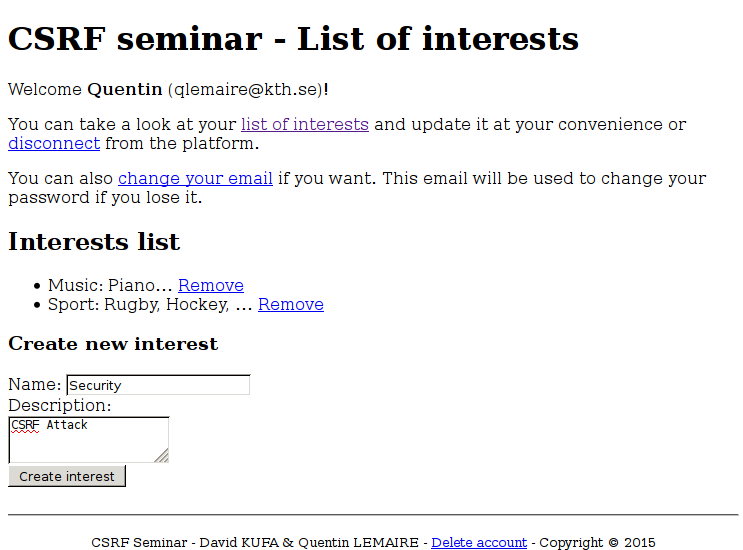
\includegraphics[width=.9\linewidth]{screens/interests.png}}
    \caption{Interests page}
    \label{figure:interests}
  \end{center}
\end{figure}
  
\begin{figure}[ht!]
  \begin{center}
    \fbox{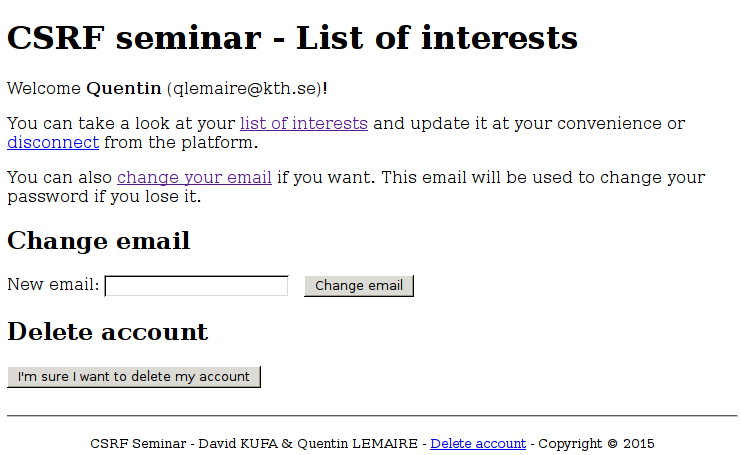
\includegraphics[width=.9\linewidth]{screens/account.png}}
    \caption{Account page}
    \label{figure:account}
  \end{center}
\end{figure}
  
% bibliography
\bibliographystyle{plainurl}
\bibliography{references}

\end{document}